\documentclass[main-physics.tex]{subfiles}

\setlength{\fboxsep}{0pt}

\usepackage{fancyhdr}
\pagestyle{fancy}
\renewcommand{\headrulewidth}{0pt}
\renewcommand{\headruleskip}{0mm}
\fancyhead{}
\def\openstax{https://openstax.org/books/physics/pages/1-introduction}
\def\openstaxfooter{\fancyfoot[C]{Access for free at \href{\openstax}{\openstax} \hfill \thepage}}

\openstaxfooter


\begin{document}

\setcounter{section}{5} % Comment out if recompiling from main-physics.tex
\section{Two-Dimensional Motion Application}

In this unit, we explore two types of two-dimensional motion: projectile motion and uniform circular motion (UCM). The first 10 lessons address projectile motion; the last 8 lessons, UCM.

\begin{mdframed}[backgroundcolor=black!10]
\textbf{Note on Section Numbering}\\
Subsections are labeled according to the Day in the Lesson Plan of this unit. For example, Section \ref{tMF7JY} corresponds to Day 3 of Unit 6.
\end{mdframed}

\vspace{1ex}

\cyanhrule

\vspace{1em}

\Gls{projectile motion} is the motion of an object thrown (projected) into the air when, after the initial force that launches the object, air resistance is negligible and the only other force that object experiences is the force of gravity. The object is called a \gls{projectile}, and its path is called its \gls{trajectory}. \Gls{air resistance} is a frictional force that slows its motion and can significantly alter the trajectory of the motion. Due to the difficulty in calculation, only situations in which the deviation from projectile motion is negligible and \textit{air resistance can be ignored} are considered in this unit. That approximation is often quite accurate.

\vspace{1em}

\begin{center}
    \begin{tikzpicture}[declare function={t(\x)=\x/(\vi*cos(\thetai));}]
    \tikzmath{
        \grav = 10;
        \vi = 20;
        \yi = 0;
        \thetai = 45.0;
        \viy = \vi*sin(\thetai);
        \ymax = (\viy^2)/(2*\grav);
        \tmax = 2*\ymax/\viy;
        \vix = \vi*cos(\thetai);
        \xmax = \vix*\tmax;
        \sf = 0.3; %scale factor for vector components
    }
    % \pgfplotsset{compat=1.11}
        \begin{axis}[width=16cm,height=9cm,ticks=none,
        axis lines = none,
        clip=false,
        ylabel = $y$,
        xlabel = $x$,
        xmin=0, xmax=50,
        ymin=0, ymax=15,
        ]
        \draw[red,domain=0:45,samples=100,variable=\x] plot(\x,{patheqten(\x,0,20,45)});
        \draw[->] (0,0) -- ++(\vix*\sf,\viy*\sf) node[above=3mm,pos=0.8] {$v_0$};
        \draw[dashed,->] (0,0) -- ++(0,{\sf*\vi*sin(\thetai)}) node[above] {$v_{0y}$};
        \draw[dashed,->] (0,0) -- ++(\vix*\sf,0) node[right] {$v_{0x}$};

        \draw[fill=black] (\xmax,\ymax) circle (2pt);
        \draw[thick,->] (\xmax,\ymax) -- ++(\vix*\sf,0);
        
        \pgfplotsinvokeforeach{0,5,10,15,25,30,35,40,45}{
                \draw[fill=black] (#1,{patheqten(#1,0,20,45)}) circle (2pt);
                \draw[dashed,->] (#1,{patheqten(#1,0,20,45)}) -- ++(0,{\sf*(\vi*sin(\thetai) - \grav*t(#1))});
                \draw[dashed,->] (#1,{patheqten(#1,0,20,45)}) -- ++(\vix*\sf,0);
                \draw[thick,->] (#1,{patheqten(#1,0,20,45)}) -- ++(\vix*\sf,{\sf*(\vi*sin(\thetai) - \grav*t(#1))});
                }
        \end{axis}
    \end{tikzpicture}
\end{center}


\clearpage
\subsection{Relevant Application: Factors that Affect Path and Hang Time} \label{1hGIbN}

\begin{mdframed}[backgroundcolor=Green!10]
    \textbf{Warm-Up}. Access the \texttt[red]{PhET Simulation} ``Projectile Motion'' (\href{https://phet.colorado.edu/sims/html/projectile-motion/latest/projectile-motion_all.html}{click here}). Click the \texttt[red]{Lab} panel. Locate the following three functions on your screen: the fire button, the first measuring tool, and the reset button, which are shown below:
\end{mdframed}

\begin{center}
    \begin{tikzpicture}
        \draw (0,0) node {\fbox{
\includegraphics[width=2cm]{physics/figures/phet-projectile-motion-2.png}}} node[above=9mm]{\texttt[red]{Fire button}};
    \end{tikzpicture}%
    \hspace{5mm}
    \begin{tikzpicture}
        \draw (0,0) node {\fbox{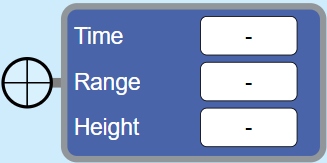
\includegraphics[width=4cm]{physics/figures/phet-projectile-motion.png}}} node[above=1cm]{\texttt[red]{Tool \#1}};
    \end{tikzpicture}
    \hspace{5mm}
    \begin{tikzpicture}
        \begin{scope}
            \clip (0,-0.03) circle (0.87);
            \draw (0,0) node {\fbox{
\includegraphics[width=2cm]{physics/figures/phet-projectile-motion-3.png}}};
            \draw[thick] (0,-0.03) circle (0.85);
        \end{scope}
        \node[above=8mm] at (0,0) {\texttt[red]{Reset button}};
    \end{tikzpicture}
\end{center}

When you press the \texttt[red]{Fire} button, a projectile is launched through the air. The path of the projectile, which is indicated by the blue curve, is called the trajectory. Three points on the trajectory are worth mentioning. First, the origin is where the cannon is positioned. Second, the maximum height occurs when the projectile reaches its largest vertical displacement. Third, maximum range occurs when the projectile impacts the ground. The \texttt[red]{Tool \#1} measures time, range, and height at several points on the path of the projectile. \texttt[red]{Time} is the time elapsed since the launch of the projectile, \texttt[red]{Range} is the projectile's horizontal displacement from the origin, and \texttt[red]{Height} is the projectile's vertical displacement from the origin. 

\begin{center}
    \begin{tikzpicture}[
        declare function={R(\vi,\thetai) = \vi^2 * sin(2*\thetai) / \grav;}, % maximum range
        declare function={h(\vi,\thetai) = (\vi*sin(\thetai))^2/(2*\grav);} %maximum height
    ]
    \tikzmath{
        \grav=9.8;
    }
    \pgfplotsset{compat=1.11}
        \begin{axis}[width=6cm,height=6cm,ticks=none,
        axis lines = center,
        axis line style={draw=none},
        clip=false,
        xmin=0, xmax={R(18,80)*1.1},
        ymin=0, ymax={h(18,80)*1.1},
        ]
        \draw[thick,RoyalBlue,domain=0:{R(18,80)},variable=\x,samples=200] plot ({\x},{patheq(\x,0,18,80)});
        \node[left] at (0,0) {origin};
        \node[rotate=72,RoyalBlue] at (2,7) {trajectory};
        \draw (0.6,0) arc (0:35:2) node[pos=1.2,right=2mm,align=left] {launch\\ angle};
        \draw[<->,dashed] (0,0) -- ++(axis direction cs: {R(18,80)},0) node[pos=0.8,below] {maximum range};
        \draw[<->,dashed] ({R(18,80)/2},0) -- ++(axis direction cs: 0,{h(18,80)}) node[above] {maximum height};
        \end{axis}
    \end{tikzpicture}
\end{center}

\vspace{1em}

\textbf{Part I: Measuring Time, Range, and Height}

\begin{enumerate}
    \item Click the \texttt[red]{Fire} button to launch a cannonball from the cannon. Observe that the path of the projectile is indicated by the blue curve. A projectile's path is called the trajectory.
    \item Draw a sketch of the trajectory. 
    \item \label{VSHLLm} Use \texttt[red]{Tool \#1} to measure time, range, and height data throughout the trajectory at 0.4-second time intervals. In other words, at times $t=\SI{0.0}{s}$, \SI{0.4}{s}, \SI{0.8}{s}, \ldots, \SI{3.6}{s}. Label your data on the sketch from Step \ref{VSHLLm}.
    \item Record time, range, and height at these three points: the origin, at maximum height, and at maximum range.
\end{enumerate}



\vspace{1em}

\textbf{Part II: How Mass Affects Projectile Path}

\begin{enumerate}
    \item The \texttt[red]{Reset} button ($\boldsymbol{\circlearrowleft}$) is located at the bottom right corner. It resets all settings to the default, as you found the page when you first opened it. Click the $\boldsymbol{\circlearrowleft}$ button.
    \item Click the \texttt[red]{Fire} button to launch a cannonball. Observe the same path, or trajectory, as before.
    \item \label{thVv3G} The default mass of the cannonball is \SI{17.60}{kg}. Change the mass to \SI{3.00}{kg}, and fire the cannon again. Did the trajectory change? Record your observations. 
    \item Repeat Step \ref{thVv3G} using the following projectile masses: $m=\SI{10}{kg}$, \SI{25}{kg}, and \SI{31}{kg}. Record your observations for each case. Then answer the following question: How does changing the mass of a projectile affect its path?
\end{enumerate}

\vspace{1em}

\textbf{Part III: How Launch Height Affects Projectile Path}
\begin{enumerate}
    \item Click the \texttt[red]{Reset} ($\boldsymbol{\circlearrowleft}$) button.
    \item Click the \texttt[red]{Fire} button, noting the familiar trajectory in blue.
    \item Locate the cannon at the origin. The values \SI{0}{m} and \ang{80} next to the cannon indicate that the projectile is set to be launched from a height of zero meters and at angle of \ang{80} from the horizontal.
    \item Locate the $\boldsymbol{+}$ symbol on the center of the cannon. Clicking and dragging this symbol upwards increases the launch height of the projectile. Change the launch height to 3 meters, fire the projectile at this height, and observe the new projectile path. Record your observations.
    \item Click-and-drag the $\boldsymbol{+}$ to change the launch height from 0 to 15 meters in increments of 3. In other words, from launch heights of \SI{0}{m}, \SI{3}{m}, \SI{6}{m}, \ldots, \SI{15}{m}. At each launch height, \texttt[red]{Fire} the projectile to observe the new trajectory. Record all your observations. 
    \item How does changing the launch height affect the path of a projectile? You may draw several sketches and use time, range, and height data from \texttt[red]{Tool \#1} to support your answer.
\end{enumerate}

\vspace{1em}

\subsection{Relevant Application ({\small \textit{cont}.}): Launch Angle and Projectile Path}

\begin{mdframed}[backgroundcolor=Green!10]
    \textbf{Warm-Up}: See Warm-Up from Section \ref{1hGIbN}.
\end{mdframed}

\textbf{Part IV: How Launch Velocity Changes Projectile Path}

\begin{enumerate}
    \item Click $\boldsymbol{\circlearrowleft}$ to reset all settings.
    \item \texttt[red]{Fire} the projectile at the default settings and observe the now-familiar trajectory. 
    \item By default, the cannon is set to fire the projectile with an initial speed (or velocity) of 18 meters per second. Decrease the velocity to \SI{12}{m/s}, \texttt[red]{Fire} the projectile, and observe the new projectile path.
    \item Increase the speed to \SI{24}{m/s}, \texttt[red]{Fire} the projectile, and observe the new trajectory.
    \item What initial speed causes the projectile to land closest to the bullseye (all other factors being equal)?
    \item How does changing launch velocity affect the path of a projectile? Draw sketches and reference time, range, and height data from \texttt[red]{Tool \#1} to support your answer.
\end{enumerate}

\vspace{1em}

\clearpage

\textbf{Part V: Launch Angle, Trajectory, and Hang Time}

\begin{enumerate}
    \item Click $\boldsymbol{\circlearrowleft}$ to reset all settings.
    \item Click-and-drag near the barrel-end of the cannon (away from the $\boldsymbol{+}$ sign) to change the cannon's launch angle. Set the angle to \ang{30}, and don't change any other settings. Press \texttt[red]{Fire} to launch the cannonball. 
    \item Let's define \texttt[red]{hang time} as the total time elapsed between the launch of the projectile and the instant it strikes the ground. To measure hang time, locate the last data point on the trajectory (i.e., the blue curve), and use \texttt[red]{Tool \#1} to view the elapsed time at the end of the curve. Record the hang time.
    \item Increase the launch angle from \ang{30} to \ang{90} in increments of \ang{10}---in other words, as \ang{30}, \ang{40}, \ldots, \ang{90}. For each angle, record the projectile's hang time.
    \item How does changing the launch angle incrementally from \ang{30} to \ang{90} affect the shape of the trajectory, including maximum height and range?
    \item How does changing launch angles affect the hang time?  
    \item Which angle yields the largest possible maximum range? You may need to try launching the projectile at a variety of angles by trial-and-error to arrive at your conclusion.
\end{enumerate}

\subsection{Vertical \& Horizontal Vectors of Position, Velocity, and Acceleration} \label{tMF7JY}

\begin{mdframed}[backgroundcolor=Green!10]
    \textbf{Warm-Up}. List what you know about the following quantities, including their SI units. Then, list what you want to know about them in two-dimensional motion.

    \begin{center}
        \textbf{position} \hspace{2em}
        \textbf{velocity} \hspace{2em}
        \textbf{acceleration}
    \end{center}
\end{mdframed}


\vspace{1em}

The most important concept in projectile motion is that when air resistance is ignored, horizontal and vertical motions are independent, meaning that they don't influence one another. Figure \ref{lTQ6jX} compares a cannonball in free fall (in red) to a cannonball launched horizontally in projectile motion (in black). You can see that \textit{the cannonball in free fall falls at the same rate as the cannonball in projectile motion}. Keep in mind that if the cannon launched the ball with any vertical component to the velocity, the vertical displacements would not line up perfectly.

\vspace{1em}

Since vertical and horizontal motions are independent, we can analyze them separately, along perpendicular axes. To do this, we separate projectile motion into the two components of its motion, one along the horizontal axis and the other along the vertical.

\begin{center}
    \begin{tikzpicture}
        \begin{axis}[width=10cm,height=10cm,ticks=none,
        axis lines = center,
        axis line style={draw=none},
        clip=false,
        % ylabel = $y$,
        % xlabel = $x$,
        xmin=0, xmax=120,
        ymin=0, ymax=70,
        ]
        \draw[dashed,domain=0:100,variable=\x,samples=200] plot ({\x},{patheq(\x,60,28.6,0)});
        \draw[dashed] (0,{patheq(0,60,28.6,0)}) -- ++(100,0);
        \draw[dashed] (0,{patheq(0,60,28.6,0)}) -- ++(0,-{patheq(0,60,28.6,0)});

        \fill (0,{patheq(0,60,28.6,0)}) circle (3pt);
        
        \pgfplotsinvokeforeach{20,40,60,80,100}{
            \fill (#1,{patheq(#1,60,28.6,0)}) circle (3pt);
            \draw[dashed] (#1,{patheq(0,60,28.6,0)}) -- ++(0,{-(patheq(0,60,28.6,0)-patheq(#1,60,28.6,0))});
            \fill[cyan] (#1,{patheq(0,60,28.6,0)}) circle (3pt);
            \draw[dashed] (0,{patheq(#1,60,28.6,0)}) -- ++(#1,0);
            \fill[red] (0,{patheq(#1,60,28.6,0)}) circle (3pt);
        }
        \begin{scope}[shift={(-10,59.4)}]
            \draw[very thick,black!80] (0,0) -- (-5,-2);
            \draw[fill=black] (-4,0) rectangle ++(8,1.2);
            \draw[fill=black] (0,0.2) rectangle ++(7,0.8);
            \draw (0,0) node {\Large\textlinb{\BPwheel}};
        \end{scope}

        \draw[fill=black!30] (-6,0) rectangle ++(-10,57.2);
        \end{axis}
    \end{tikzpicture}
    \captionsetup{type=figure,margin=1in,font=scriptsize}
    \captionof{figure}{The diagram shows the projectile motion of a cannonball shot at a horizontal angle versus one dropped with no horizontal velocity. Note that both cannonballs have the same vertical position over time.}
    \label{lTQ6jX}
\end{center}

\vspace{1em}

We'll call the horizontal axis the $x$-axis and the vertical axis the $y$-axis. For notation, $d$ is the total displacement, and $x$ and $y$ are its components along the horizontal and vertical axes. The magnitudes of these vectors are $x$ and $y$, as illustrated in Figure \ref{i1Y7vV}.

\begin{center}
    \begin{tikzpicture} 
        \begin{axis}[width=8cm,height=8cm,ticks=none,
            axis lines = center,
            clip=false,
            ylabel = $y$,
            xlabel = $x$,
            xmin=0, xmax=20,
            ymin=0, ymax=18,
        ]
        \node at (15.6,0.35) {$\square$};
        \draw[dashed,domain=0:16,variable=\x,samples=200] plot ({\x},{patheq(\x,0,18,70)}) node[above left=-4pt] {\faSoccerBallO};
        \draw[->,thick] (0,0) -- ++(16,{patheq(16,0,18,70)}) node[pos=0.5,above=3pt]{$d$};
        \draw[->,dashed,ultra thick,RoyalBlue] (0,0) -- ++(16,0) node[pos=0.5,below] {$x$};
        \draw[->,dashed,ultra thick,red] (16,0) -- ++(0,{patheq(16,0,18,70)}) node[pos=0.5,right] {$y$};
        \node at (2.5,0.65) {$\theta$};
        \draw (1.5,0) arc (0:35:1.5);
        \draw (0,0) node[left] {\Strichmaxerl[3]};
        \end{axis}
    \end{tikzpicture}
    \captionsetup{type=figure,margin=1in,font=scriptsize}
    \captionof{figure}{A boy kicks a ball at angle $\theta$, and it is displaced a distance of $d$ along its trajectory.}
    \label{i1Y7vV}
\end{center}

\subsubsection*{\ref{tMF7JY} Exercises}

\begin{exercise} \label{KU3Mnf}
Access the \texttt[red]{PhET Simulation} ``Projectile Motion'' (\href{https://phet.colorado.edu/sims/html/projectile-motion/latest/projectile-motion_all.html}{click here}). Click the \texttt[red]{Vectors} panel, and take the following steps:

\begin{enumerate}
    \item Un-check the \texttt[red]{Air Resistance} box. (Leave it blank.)
    \item Raise the cannon to a height of \SI{11}{m}, change the launch angle to \ang{0} for a horizontal launch, and decrease the \texttt[red]{Initial Speed} to \SI{10}{m/s}.
    \item Click the \texttt[red]{Components} option, and check the \texttt[red]{Velocity Vectors} box.
    \item Press \texttt[red]{Pause} (\small \faPause).
    \item Press the \texttt[red]{Fire} button. The initial velocity, which is entirely horizontal is displayed. Notice that vertical velocity is not shown because it's zero.
    \item Sketch the horizontal and vertical velocity vectors of this snapshot in a motion map. 
    \item To the right of the \texttt{Play} ({\small \faPlay}) button there is the \texttt[red]{Step} ({\small \mystep}) button. Press the \texttt[red]{Step} button several times to view the evolution of the horizontal and vertical velocity vectors. 
    \item \label{LSagnx} Using {\small \mystep}, draw the the horizontal and vertical components of velocity in your motion map at 3 to 4 instances between the projectile being fired and its striking the ground.
\end{enumerate}
\end{exercise}

\begin{exercise}
    Repeat Step \ref{LSagnx} of Exercise \ref{KU3Mnf}, drawing horizontal and vertical velocity components at 7 to 8 instances, but this time launch the cannon from ground level ($\text{height} = 0$), at an launch angle of \ang{70}, with an initial speed of \SI{15}{m/s}. Be sure to include the first point, the last point, and the point at which the projectile is at maximum height. Compare your finalized sketch to Figure \ref{xRbMxN}.
\end{exercise}

\begin{exercise} \label{nmtty2}
    What is projectile motion?
    
    \begin{enumerate}[label=\Alph*.]
        \item Projectile motion is the motion of an object projected into the air and moving under the influence of gravity.
        \item Projectile motion is the motion of an object projected into the air and moving independently of gravity.
        \item Projectile motion is the motion of an object projected vertically upward into the air and moving under the influence of gravity.
        \item Projectile motion is the motion of an object projected horizontally into the air and moving independently of gravity.
    \end{enumerate}
\end{exercise}

\begin{exercise} \label{uLtw6P}
    What is the force experienced by a projectile after the initial force that launched it into the air in the absence of air resistance?

    \begin{enumerate}[label=\Alph*.]
        \item The nuclear force
        \item The gravitational force
        \item The electromagnetic force
        \item The contact force
    \end{enumerate}
\end{exercise}

\begin{exercise} \label{sy5RGT}
    After a projectile is launched in the air, in which direction does it experience constant, non-zero acceleration, ignoring air resistance?

    \begin{enumerate}[label=\Alph*.]
        \item The x direction
        \item The y direction
        \item Both the x and y directions
        \item Neither direction
    \end{enumerate}
\end{exercise}

\begin{exercise} \label{90PABl}
    What is the angle between the $x$ and $y$ components of a vector?

    \begin{enumerate}[label=\Alph*.]
        \item \ang{0}
        \item \ang{90}
        \item \ang{45}
        \item \ang{180}
    \end{enumerate}
\end{exercise}

\begin{exercise} \label{8I1QP6}
    Horizontal and vertical motions of a projectile are independent of each other. What does this mean?

\begin{enumerate}[label=\Alph*.]
    \item All objects in projectile motion with the same initial vertical velocity fall at the same rate, regardless of their horizontal velocity.
    \item All objects in projectile motion fall at different rates, regardless of their initial horizontal velocities.
    \item Any object in projectile motion falls at the same rate as its initial vertical velocity, regardless of its initial horizontal velocity.
    \item All objects in projectile motion fall at different rates and the rate of fall of the object is independent of the initial velocity.
\end{enumerate}
\end{exercise}

\begin{center}
    \begin{tikzpicture}[declare function={t(\x)=\x/(\vi*cos(\thetai));}]
    \tikzmath{
        \grav = 10;
        \vi = 20;
        \yi = 0;
        \thetai = 45.0;
        \viy = \vi*sin(\thetai);
        \ymax = (\viy^2)/(2*\grav);
        \tmax = 2*\ymax/\viy;
        \vix = \vi*cos(\thetai);
        \xmax = \vix*\tmax;
        \sf = 0.3; %scale factor for vector components
    }
    % \pgfplotsset{compat=1.11}
        \begin{axis}[width=16cm,ticks=none,
        axis lines = none,
        clip=false,
        ylabel = $y$,
        xlabel = $x$,
        xmin=0, xmax=50,
        ymin=0, ymax=15,
        ]
        \draw[gray,->] (0,0) -- ++(0,10) node[right] {$y$};
        \draw[gray,->] (0,0) -- ++(48,0) node[above] {$x$};
        \draw[fill=black] (0,0) circle (2pt);
        \draw[thick,violet,->] (0,0) -- ++(\vix*\sf,\viy*\sf) node[below right] {$v_0$};
        \draw[thick,dashed,red,->] (0,0) -- ++(0,{\sf*\vi*sin(\thetai)}) node[right=-2pt] {$v_{0y}$};
        \draw[thick,dashed,RoyalBlue,->] (0,0) -- ++(\vix*\sf,0) node[pos=1.3, above=-2pt] {$v_{0x}$};
        \draw (1,0) arc (0:75:0.6) node[midway,right=-1pt] {$\theta_0$};
        
        \pgfplotsinvokeforeach{5,10,15}{
                \draw[fill=black] (#1,{patheqten(#1,0,20,45)}) circle (2pt);
                \draw[thick,dashed,red,->] (#1,{patheqten(#1,0,20,45)}) -- ++(0,{\sf*(\vi*sin(\thetai) - \grav*t(#1))}) node[above=-2pt] {$v_y$};
                \draw[thick,dashed,RoyalBlue,->] (#1,{patheqten(#1,0,20,45)}) -- ++(\vix*\sf,0) node[right=-2pt] {$v_x$};
                \draw[thick,violet,->] (#1,{patheqten(#1,0,20,45)}) -- ++(\vix*\sf,{\sf*(\vi*sin(\thetai) - \grav*t(#1))}) node[above=-2pt] {$v$};
                }
                
        \draw[fill=black] (\xmax,\ymax) circle (2pt);
        \draw[thick,violet,->] (\xmax,\ymax) -- ++(\vix*\sf,0) node[right=-2pt] {$v = v_x$};
        
        \pgfplotsinvokeforeach{25,30,35,45}{
                \draw[fill=black] (#1,{patheqten(#1,0,20,45)}) circle (2pt);
                \draw[thick,dashed,red,->] (#1,{patheqten(#1,0,20,45)}) -- ++(0,{\sf*(\vi*sin(\thetai) - \grav*t(#1))}) node[below=-2pt] {$v_y$};
                \draw[thick,dashed,RoyalBlue,->] (#1,{patheqten(#1,0,20,45)}) -- ++(\vix*\sf,0) node[right=-2pt] {$v_x$};
                \draw[thick,violet,->] (#1,{patheqten(#1,0,20,45)}) -- ++(\vix*\sf,{\sf*(\vi*sin(\thetai) - \grav*t(#1))}) node[below=-2pt] {$v$};
                }

                \draw[fill=black] (40,{patheqten(40,0,20,45)}) circle (2pt);
                \draw[thick,dashed,red,->] (40,{patheqten(40,0,20,45)}) -- ++(0,{\sf*(\vi*sin(\thetai) - \grav*t(40))}) node[left=-2pt] {$v_y=-v_{0y}$};
                \draw[thick,dashed,RoyalBlue,->] (40,{patheqten(40,0,20,45)}) -- ++(\vix*\sf,0) node[above=-2pt] {$v_x$};
                \draw[thick,violet,->] (40,{patheqten(40,0,20,45)}) -- ++(\vix*\sf,{\sf*(\vi*sin(\thetai) - \grav*t(40))}) node[below=-2pt] {$v$};
                % \draw (40.8,0) arc (0:-\thetai:0.8) node[midway,right=-1pt] {$\theta =-\theta_0$};
                \draw (5.8,{patheqten(5,0,20,45)}) arc (0:40:0.8) node[midway,right] {$\theta$};
        \end{axis}
    \end{tikzpicture}
    \captionsetup{type=figure,font=scriptsize}
    \captionof{figure}{We analyze two-dimensional projectile motion by breaking it into two independent one-dimensional motions along the vertical and horizontal axes. The horizontal motion is constant. The velocity in the vertical direction begins to decrease, then becomes zero at the peak, then increases in the downward direction.}
    \label{xRbMxN}
\end{center}


\subsection{Describing Vertical and Horizontal Motion}

\begin{mdframed}[backgroundcolor=Green!10]
    \textbf{Warm-Up}. Exercises \ref{MbIMKN}, \ref{tnuYO3}, and \ref{ObtV91}.

    \vspace{1em}
    
    A boulder is dropped from rest from the top of a tall cliff. The boulder accelerates downwards at a rate of \SI{10}{m/s^2}.

    \begin{exercise} \label{MbIMKN}
        Create a table listing the boulder's speed at times $t = \SI{0}{s}$, \SI{1}{s}, \SI{2}{s}, \SI{3}{s}, \SI{4}{s}, and \SI{5}{s} after being dropped.
    \end{exercise}

    \begin{exercise} \label{tnuYO3}
        The bolder has a mass of \SI{5}{kg}. (a) What is it's initial momentum? (b) What is its initial kinetic energy?
    \end{exercise}

    \begin{exercise} \label{ObtV91}
        (a) Calculate the momentum of the 5-kg boulder 3 seconds into its free fall. (b) Calculate its kinetic energy at $t = \SI{1}{s}$.
    \end{exercise}
\end{mdframed}




As usual, we use velocity, acceleration, and displacement to describe motion. We must also find the components of these variables along the $x$- and $y$-axes. The components of acceleration are then very simple. In the vertical direction,

\begin{equation}
    a_y = -g = -\SI{10}{m/s^2}
\end{equation}

Note that this definition defines the upwards direction as positive. In the horizontal direction, because gravity is vertical only,

\begin{equation}
    a_x = 0
\end{equation}

Both accelerations are constant, so we can use the kinematic equations. For review, the kinematic equations from previous units are summarized below.

\begin{align}
    x &= x_0 + v_{\text{avg}} t\\[0.5ex]
    v_{\text{avg}} &= \frac{v_0 + v}{2}\\[0.5ex]
    v &= v_0 + a t\\[0.5ex]
    x &= x_0 + v_0 t + \frac{1}{2} a t^2\\[0.5ex]
    v^2 &= v_0^2 + 2 a (x - x_0)
\end{align}

where $x$ is position, $x_0$ is initial position, $v$ is velocity, $v_{\text{avg}}$ is average velocity, $t$ is time, and $a$ is acceleration.

\subsection{How to Set-Up and Analyze Projectile Motion Problems}

The following four steps are used to analyze projectile motion:

\vspace{1em}

\textbf{Step 1}: Know what each of the many variables means; see Table \ref{zvgNdH}. Recall that a variable is used to represent a physical quantity. The magnitudes of the displacement $d$ along $x$- and $y$-axes are called $x$ and  $y$. The magnitude of the velocity is $v$, and the magnitudes of the components of the velocity, $v_x$ and $v_y$, relate to $v$ also by the Pythagorean theorem. Initial values are denoted with a subscript 0.

\vspace{1em}

\textbf{Step 2}: Treat the motion as two independent one-dimensional motions, one horizontal and the other vertical. The kinematic equations for horizontal motion take the following forms under the condition that horizontal acceleration is zero ($a_x = 0$):

\begin{align}
    x &= x_0 + v_x t \label{7fMAPG}\\[0.5ex]
    v_x &= v_{0x} = \text{velocity is a constant} \label{dCvDf4}
\end{align}

For vertical motion, the kinematic equations take the following forms under the condition that vertical acceleration is $a_y = -g = \SI{-10}{m/s^2}$:

\begin{align}
    y &= y_0 + \frac{1}{2}\left(v_{0y} + v_y\right)t\\[0.5ex]
    v_y &= v_{0y} - gt \label{SjYaoE} \\[0.5ex]
    y &= y_0 + v_{0y}t - \frac{1}{2}  g t^2  \label{36YuvF} \\[0.5ex]
    % v_y^2 &= v_{0y}^2 - 2 g (y - y_0) \label{wROSXN}
\end{align}

\vspace{1em}

\textbf{Step 3}: Solve for the unknowns in the two separate motions (one horizontal and one vertical). Note that the only common variable between the motions is time $t$. The problem solving procedures here are the same as for one-dimensional kinematics.

\vspace{1em}

\textbf{Step 4}: Recombine the two motions to find the total displacement $d$ and velocity $v$. These are related to their components via the Pythagorean theorem as shown below:

\begin{align}
    d &= \sqrt{x^2 + y^2} \label{XvIie8} \\[0.5ex]
    v &= \sqrt{v_x^2 + v_y^2} \label{glASeI}
\end{align}

\begin{mdframed}[backgroundcolor=black!10]
    \textbf{Tips For Success}\\
    For problems of projectile motion, it is important to set up a coordinate system. The first step is to choose an initial position for $x$ and $y$. Usually, it is simplest to set the initial position of the object so that $x_0 = 0$ and $y_0 = 0$.
\end{mdframed}

\vspace{1em}

\begin{center}
    \begin{tabular}{cl|cl}
    \hline
    \textbf{Symbol} & \textbf{Quantity} & \textbf{SI Unit} & \textbf{Unit Symbol}  \\
    \hline\hline
        $d$ & displacement from origin & meter & m\\
        $x$ & horizontal component of displacement & meter & m\\
        $y$ & vertical component of displacement & meter & m\\
        $v$ & instantaneous velocity & meter per second squared & m/s\\
        $v_x$ & horizontal component of velocity & meter per second squared & m/s\\
        $v_y$ & vertical component of velocity & meter per second squared & m/s\\
        $a_y$ & vertical component of acceleration & meter per second squared & \SI{}{m/s^2}\\ 
        $a_x$ & horizontal component of acceleration & meter per second squared & \SI{}{m/s^2}\\
        $t$ & time & second & s\\
        $g$ & acceleration due to gravity & meter per second squared & \SI{}{m/s^2}\\
        $\theta$ & launch angle & degrees & \SI{}{\degree}\\
    \hline
    \end{tabular}
\captionsetup{type=table,margin=1in,font=scriptsize}
\captionof{table}{Summary of physical quantities in projectile motion, the variables that represent them, and their SI units. Initial values are denoted with a subscript 0, as, for example, $y_0$ and $v_{0x}$. Note: displacement $d$ and components $x$ and $y$ are defined under the assumption that $x_0$ and $y_0$ are zero.}
\label{zvgNdH}
\end{center}




\clearpage




\begin{example} \label{ER19WG}
    Suppose the cannonball from Figure \ref{lTQ6jX} is launched horizontally from a height of \SI{12.0}{m} at a speed of \SI{18.0}{m/s}. How much time will it take the projectile to strike the ground?
\end{example}

\Solution Our strategy is based on the fact that the motion can be broken into horizontal and vertical motions in which $a_x = 0$ and $a_y = \SI{-10}{m/s^2}$. Start by drawing a sketch:

\begin{center}
    \begin{tikzpicture}
        \begin{axis}[width=7cm,height=7cm,
            ticks=none,
            xmin=0,xmax=32,
            ymin=0,ymax=15,
            clip=false,
            axis lines=left,
        ]
            \draw[RoyalBlue,domain=0:28.15,variable=\x,samples=100] plot(\x,{patheq(\x,12,18,0)}) node[black,below] {$t =\ ?$} node[black,below=4mm] {\StopWatchEnd}; 
            \fill (0,{patheq(0,12,18,0)}) circle (3pt) node[left=2pt] {$t_0 = 0$} node[below left=2mm] {\StopWatchStart};
            \draw[red,thick,->] (0,{patheq(0,12,18,0)}) -- ++(6,0) node[right] {\SI{18}{m/s}};
            \draw[<->,dashed] (1,0) -- ++(0,12) node[right,pos=0.5] {\SI{12}{m}};
        \end{axis}
    \end{tikzpicture}
\end{center}


Let's define given variables and the unknown. First, define initial positions as 

\begin{equation*}
    x_0 = \SI{0}{m} \quad \text{and} \quad y_0 = \SI{0}{m}
\end{equation*}

Thus, the cannonball's final vertical position will be

\begin{equation*}
    y = -\SI{12}{m}
\end{equation*}

(the negative sign indicating that the projectile will be displaced downwards at the moment of impact). In addition, if a projectile is horizontally launched, then the vertical component of its initial velocity is zero:

\begin{equation*}
    v_{0y} = 0
\end{equation*}

The unknown variable is time: $t =\ ?$ These given and unknown variables are related by Equation \eqref{36YuvF}:

\begin{equation*}
    y = y_0 + v_{0y}t - \frac{1}{2}  g t^2 
\end{equation*}

Substituting known and unknown values leads to

\begin{equation*}
    -12 = 0 + (0) t - \frac{1}{2} (10) t^2
\end{equation*}

or, more simply, to

\begin{equation*}
    -12 = -5 t^2
\end{equation*}

Furthermore, multiplying both sides by $-1$ results in the negative signs canceling out, leaving

\begin{equation*}
    12 = 5 t^2
\end{equation*}

To finish solving this equation for time ($t$), we take the following steps:

\begin{align*}
    \textbf{Write $t$ on left} \qquad & 5 t^2 = 12\\[1ex]
    \textbf{Divide by 5} \qquad & \frac{\cancel{5} t^2}{\textcolor{red}{\cancel{5}}} = \frac{12}{\textcolor{red}{5}}\\[1ex]
    \textbf{Simplify} \qquad & t^2 = \frac{12}{5}\\[1ex]
    \textbf{Simplify} \qquad & t^2 = 2.4\\[1ex]
    \textbf{Take square root} \qquad & \sqrt{t^2} = \sqrt{2.4}\\[1ex]
    \textbf{Simplify} \qquad & t = 1.5
\end{align*}

Therefore, it takes the cannonball 1.5 seconds after being launched by the cannon to strike the ground below. 

\endsolution

\subsection{Solving Problems in Projectile Motion \texttt{(PART I)}}

\begin{example} \label{jKndVF}
    What is the range of the projectile from Example \ref{ER19WG}? (Calculate the horizontal displacement from its origin.)
\end{example}

\Solution In Example \ref{ER19WG}, we determined the initial position and hang time of the cannonball:

\begin{equation*}
    x_0 = 0 \quad \text{and} \quad t = \SI{1.5}{s}
\end{equation*}

Also, we were given an initial horizontal velocity of \SI{18}{m/s}, and Equation \eqref{dCvDf4} implies that this horizontal velocity of the cannonball remains the same throughout the trajectory:

\begin{equation*}
    v_x = v_{0x} = \text{velocity is a constant} = \SI{18.0}{m/s}
\end{equation*}

The unknown variable is range, or horizontal displacement, which in this case is given by Equation \eqref{7fMAPG} as

\begin{equation*}
    x = x_0 + v_x t
\end{equation*}

Substituting given values leads to 

\begin{equation*}
    x = 0 + (\SI{18}{m/s})(\SI{1.5}{s}) = \SI{27}{m}
\end{equation*}

Therefore, the cannonball is horizontally displaced by 27 meters from its origin.

\endsolution

\begin{example}
    Calculate the magnitude of displacement at the instant the projectile strikes the ground, for the cannonball from Example \ref{ER19WG}.
\end{example}

\Solution In Examples \ref{ER19WG} and \ref{jKndVF}, we defined the cannonball's origin as $x_0 = 0$ and $y_0 = 0$, and we determined that the vertical and horizontal positions at the point of impact are

\begin{equation*}
    \quad x = \SI{27}{m} \quad \text{and} \quad y = \SI{-12}{m}
\end{equation*}

as shown in the figure below.

\begin{center}
    \begin{tikzpicture}
        \begin{axis}[width=7cm,height=7cm,
        ticks=none,
        axis lines = center,
        % axis line style={draw=none},
        clip=false,
        ylabel = $y$,
        xlabel = $x$,
        xmin=0, xmax=35,
        ymin=0, ymax=15,
        ]
        \draw[dashed,domain=0:28.15,variable=\x,samples=200] plot ({\x},{patheq(\x,12,18,0)});
        \fill (0,{patheq(0,12,18,0)}) circle (2pt) node[left] {$(0,0)$};
        \fill (28.15,{patheq(28.15,12,18,0)}) circle (2pt) node[below] {$(27,-12)$};
        \draw[thick,->,RoyalBlue] (0,{patheq(0,12,18,0)}) -- (28,{patheq(28,12,18,0)}) node[pos=0.5,below left] {$d$};
        \end{axis}
    \end{tikzpicture}
\end{center}

By Equation \eqref{XvIie8}, the magnitude of displacement from the origin is given by

\begin{equation*}
    d = \sqrt{x^2 + y^2}
\end{equation*}

Substituting known values leads to

\begin{equation*}
    d = \sqrt{\left(27\right)^2 + \left(-12\right)^2} = \SI{30}{m}
\end{equation*}

(rounded up from 29.5). Therefore, the magnitude of displacement is 30 meters from the origin.

\endsolution

\subsection{Solving Problems in Projectile Motion \texttt{(PART II)}}

\begin{example}
    Calculate the magnitude of velocity of the projectile from Example \ref{ER19WG} the instant it strikes the ground. This is known as the impact velocity.
\end{example}

\Solution In Example \ref{jKndVF}, we established that the horizontal component of the cannonball remains at the constant value of

\begin{equation*}
    v_x = \SI{18}{m/s}
\end{equation*}

throughout the trajectory; this is the same value as $v_{0x}$. The unknown we are looking for is magnitude of impact velocity, which is given by Equation \eqref{glASeI} as

\begin{equation*}
    v = \sqrt{v_x^2 + v_y^2}
\end{equation*}

Therefore, lets first calculate the vertical component of velocity at impact, $v_y$, which is given by Equation \eqref{SjYaoE} as

\begin{equation*}
    v_y = v_{0y} - gt
\end{equation*}

where $g = \SI{10}{m/s^2}$. A projectile that is horizontally launched implies that $v_{0y} = 0$. Also, in Example \ref{ER19WG}, we calculated the following hang time for the cannonball:

\begin{equation*}
    t = \SI{1.5}{s}
\end{equation*}

So, substituting known values into Equation \eqref{SjYaoE} leads to 

\begin{equation*}
    v_y = 0 - (\SI{10}{m/s^2})(\SI{1.5}{s}) = -\SI{15}{m/s} 
\end{equation*}

the negative sign indicating that vertical velocity is, as we expect, pointing downwards, towards the ground. Finally, substituting the given horizontal and vertical velocity components into Equation \eqref{glASeI} leads to

\begin{equation*}
    v = \sqrt{v_x^2 + v_y^2} = \sqrt{\left(\SI{18}{m/s}\right)^2 + \left(-\SI{15}{m/s}\right)^2} = \SI{23}{m/s}
\end{equation*}

Therefore, the impact velocity is 23 meters per second, below and to the right.

\begin{center}
    \begin{tikzpicture}
        \begin{axis}[width=6cm,height=6cm,
        ticks=none,
        axis lines = center,
        % axis line style={draw=none},
        clip=false,
        ylabel = $y$,
        xlabel = $x$,
        xmin=0, xmax=35,
        ymin=0, ymax=15,
        ]
        \draw[dashed,domain=0:28.15,variable=\x,samples=200] plot ({\x},{patheq(\x,12,18,0)});
        \fill (28.15,{patheq(28.15,12,18,0)}) circle (2pt);
        \draw[thick,->,red] (28.15,{patheq(28.15,12,18,0)}) -- ++(axis direction cs: 0.3*18,-0.3*15.3) node[right,black] {$v = \SI{23.6}{m/s}$};
        \end{axis}
    \end{tikzpicture}
\end{center}

\endsolution






\subsection{Exercises}

% \subsubsection*{\nameref{tMF7JY}}

\begin{exercise} \label{EykTi8}
    If an object is thrown horizontally, travels with an average $x$-component of its velocity equal to \SI{5}{m/s}, and does not hit the ground, what will be the $x$-component of the displacement after \SI{20}{s}? 

    \begin{enumerate}[label=\Alph*.]
        \item \SI{-100}{m}
        \item \SI{-4}{m}
        \item \SI{4}{m}
        \item \SI{100}{m}
    \end{enumerate}
\end{exercise}

\begin{exercise} \label{V9LJjv}
    If a ball is thrown straight up with an initial velocity of \SI{20}{m/s} upward, what is the maximum height it will reach?

    \begin{enumerate}[label=\Alph*.]
        \item \SI{-20.4}{m}
        \item \SI{-1.02}{m}
        \item \SI{1.02}{m}
        \item \SI{20.4}{m}
    \end{enumerate}
\end{exercise}

\begin{exercise} \label{YYBBp5}
    Using the conventional choice for positive and negative axes described in the text, what is the $y$-component of the acceleration of an object experiencing projectile motion?
\end{exercise}

% \begin{exercise}  \label{agp59Z}
%     Two identical items, object 1 and object 2, are dropped from the top of a \SI{50.0}{m} building. Object 1 is dropped with an initial velocity of \SI{0}{m/s}, while object 2 is thrown straight downward with an initial velocity of \SI{13.0}{m/s}. What is the difference in time, in seconds rounded to the nearest tenth, between when the two objects hit the ground?
% \end{exercise}

% \begin{exercise} \label{Xu3FK9}
%     A water balloon cannon is fired at \SI{30}{m/s} at an angle of \ang{50} above the horizontal. How far away will it fall?
% \end{exercise}

% \begin{exercise} \label{piJ9kJ}
%     A person wants to fire a water balloon cannon such that it hits a target \SI{100}{m} away. If the cannon can only be launched at \ang{45} above the horizontal, what should be the initial speed at which it is launched?
% \end{exercise}






% \begin{exercise} \label{N0Bwou}
%     A ball is thrown in the air at an angle of \ang{40}. If the maximum height it reaches is \SI{10}{m}, what must be its initial speed?
% \end{exercise}

% \begin{exercise} \label{lhjg95}
%     A large rock is ejected from a volcano with a speed of \SI{30}{m/s} and at an angle \ang{60} above the horizontal. The rock strikes the side of the volcano at an altitude of \SI{10.0}{m} lower than its starting point. Calculate the horizontal displacement of the rock.
% \end{exercise}

\begin{exercise} \label{wlbvvu}
    How can you express the velocity, $v$, of a projectile in terms of its initial velocity, $v_0$, acceleration, $g$, and time, $t$?
\end{exercise}

% \begin{exercise}
%     In the equation for the maximum height of a projectile, what does $v_{0y}$ stand for?

% \begin{equation*}
%     h = \frac{v_{0y}^2}{2g}
% \end{equation*}
% \end{exercise}

\begin{exercise} \label{xj6gln}
    True or False? Range is defined as the maximum vertical distance travelled by a projectile. 
\end{exercise}

\begin{exercise} \label{5wfdN0}
    For what angle of a projectile is its range equal to zero?
\end{exercise}

\begin{exercise} \label{DnqDpu}
    Ignoring drag, what is the $x$-component of the acceleration of a projectile? Why?
\end{exercise}

\begin{exercise} \label{QsBUvP}
    What is the optimum angle at which a projectile should be launched in order to cover the maximum distance?
\end{exercise}

\vspace{1em}

\cyanhrule

\vspace{1em}

\textbf{\ref{X0YL6f}--\ref{4gdNXl}} A pebble is launched horizontally at an initial velocity and height that are indicated in the Figure \ref{kv6ULK} below. All questions below correspond to the point at which the pebble impacts the ground $(x,y)$.

\begin{center}
    \begin{tikzpicture}
        \begin{axis}[width=6cm,height=6cm,ticks=none,
        axis lines = center,
        %axis line style={draw=none},
        clip=false,
        % ylabel = $y$,
        % xlabel = $x$,
        xmin=0, xmax=45,
        ymin=0, ymax=18,
        ]
        \draw[dashed,domain=0:40.22,variable=\x,samples=100] plot ({\x},{patheq(\x,15,23,0)});
        \draw[fill=black!25] (-0.8,0) rectangle ++(-3,15) node[pos=0.5,left=3mm] {\SI{15}{m}};
        \fill (0,{patheq(0,15,23,0)}) circle (2pt) node[above left] {$(x_0,y_0)$};
        \draw[thick,->] (0,{patheq(0,15,23,0)}) -- ++(axis direction cs: 10,0) node[right] {\SI{23}{m/s}};
        \fill (40.22,{patheq(40.22,15,23,0)}) circle (2pt) node[below] {$(x,y)$};
        \end{axis}
    \end{tikzpicture}
    \captionsetup{type=figure,margin=1in,font=scriptsize}
    \captionof{figure}{A pebble is launched from a height of 15 meters at an initial speed of 23 meters per second. It impacts the ground some time later.}
    \label{kv6ULK}
\end{center}

\begin{exercise} \label{X0YL6f}
    What is the vertical displacement?
\end{exercise}

\begin{exercise} \label{9w3tAm}
    Calculate the amount of time it takes the object to strike the ground.
\end{exercise}

\begin{exercise} \label{k9Vh0r}
    Calculate the horizontal displacement. 
\end{exercise}

\begin{exercise} \label{jCKHLv}
    What is the pebble's total displacement?
\end{exercise}

\begin{exercise} \label{4gdNXl}
    Calculate the magnitude of the pebble's impact velocity.
\end{exercise}


\cyanhrule



\clearpage

\subsection{Key Terms}

\printnoidxglossaries


\clearpage

\subsection{Answers to Select Exercises \texttt{(INSTRUCTORS ONLY)}}
\ref{EykTi8}. D. \SI{100}{m}\\
\ref{V9LJjv}. D. \SI{20.4}{m}\\
\ref{nmtty2}. A. \\
\ref{uLtw6P}. B.\\
\ref{90PABl}. \ang{90}\\
\ref{8I1QP6}. A.\\
\ref{MbIMKN}. $v = \SI{0}{m/s}$, \SI{10}{m/s}, \SI{20}{m/s}, \SI{30}{m/s}, \SI{40}{m/s}, and \SI{50}{m/s}.\\
\ref{tnuYO3}. (a) $p_0 = 0$; \hspace{1em} (b) $\text{KE}_0 = 0$\\
\ref{ObtV91}. (a) \SI{150}{kg \cdot m/s}; \hspace{1em} (b) \SI{250}{J};\\
\ref{YYBBp5}. \SI{-10}{m/s^2}\\
% \ref{agp59Z}. \SI{1.1}{s}\\
% \ref{Xu3FK9}. \SI{90.4}{m}\\
% \ref{piJ9kJ}. \SI{31.3}{m/s}\\
\ref{sy5RGT}. Vertical (or $y$)\\
% \ref{N0Bwou}. \SI{21.8}{m/s}\\
% \ref{lhjg95}. \SI{84.9}{m}\\
\ref{wlbvvu}. See Equation \eqref{SjYaoE}\\
\ref{xj6gln}. Range is horizontal.\\
\ref{5wfdN0}. \ang{0} or \ang{90}\\
\ref{DnqDpu}. \SI{0}{m/s^2}. Gravitational acceleration is vertical only.\\
\ref{QsBUvP}. \ang{45}\\
\ref{X0YL6f}. $-\SI{15}{m}$\\
\ref{9w3tAm}. \SI{1.75}{s}\\
\ref{k9Vh0r}. \SI{40.2}{m}\\
\ref{jCKHLv}. \SI{42.9}{m}\\
\ref{4gdNXl}. \SI{28.7}{m/s}





\end{document}



%%%%%%%%%%%%%%%%%%%%%%%%%%%%%%%%%%%%%%%%%%%%%%%%%%%%%%%%%%%%%%%%%%%%%%%%
%%%%%%%%%%%%%%%%%%%%%%%%%%%%%%%%%%%%%%%%%%%%%%%%%%%%%%%%%%%%%%%%%%%%%%%%
%%%%%%%%%%%%%%%%%%%%%%%%%%%%%%%%%%%%%%%%%%%%%%%%%%%%%%%%%%%%%%%%%%%%%%%%



\subsection{Uniform Circular Motion} \label{uPOucv}
\subsubsection*{Centripetal Acceleration}

Circular motion is when an object moves in a circular path. Examples of circular motion include a race car speeding around a circular curve, a toy attached to a string swinging in a circle around your head, or the circular loop-the-loop on a roller coaster. The simplest case of circular motion is \gls{uniform circular motion}, where an object travels a circular path at a constant speed. Note that, unlike speed, the linear velocity of an object in circular motion is constantly changing because it is always changing direction. We know that acceleration is a change in velocity, either in magnitude or in direction or both. Therefore, an object undergoing uniform circular motion is always accelerating, even though the magnitude of its velocity is constant.

\vspace{1em}

You experience this acceleration yourself every time you ride in a car while it turns a corner. If you hold the steering wheel steady during the turn and move at a constant speed, you are executing uniform circular motion. What you notice is a feeling of sliding (or being flung, depending on the speed) away from the center of the turn. This isn't an actual force that is acting on you---it only happens because your body wants to continue moving in a straight line (as per Newton's first law) whereas the car is turning off this straight-line path. Inside the car it appears as if you are forced away from the center of the turn. This fictitious force is known as the \gls{centrifugal force}. The sharper the curve and the greater your speed, the more noticeable this effect becomes.

\begin{center}
\begin{tikzpicture}
    \begin{axis}[
        width=7cm,height=7cm,
        axis line style={draw=none},
        ticks=none,
        axis lines=middle,
        xmin=-1,xmax=1,
        ymin=-1,ymax=1,
        clip=false,
    ]
    \draw[gray] (0,0) circle (1);
    \fill (0,0) circle (1pt);
    \fill ({cos(45)},{sin(45)}) circle (3pt) node[above right] {$m$};
    \begin{scope}[shift={(axis direction cs: 0.04,-0.04)}]
        \draw[dashed,<->] (0,0) -- ({cos(45)},{sin(45)}) node[pos=0.5,below right=-1pt] {$r$};
    \end{scope}
    \draw[Green,very thick,->] ({cos(45)},{sin(45)}) -- ++(axis direction cs: -0.3,-0.3) node[black,above=5pt,pos=1.2] {$a_{\text{c}}$};
    \draw[red,very thick,->] ({cos(45)},{sin(45)}) -- ++(axis direction cs: -0.6,0.6) node[black,pos=1.1] {$v$};
\end{axis}
\end{tikzpicture}
\captionsetup{type=figure,margin=1in,font=scriptsize}
\captionof{figure}{Uniform circular motion, the radius of curvature and vectors for tangential velocity and centripetal acceleration. Compare this with the Ladybug Motion Simulation in Exercise \ref{N066SF}.}
\label{4QmpMJ}
\end{center}

Other examples of (approximate) uniform circular motion include the \href{https://youtu.be/3NYlYN-QTig}{hammer throw}, a bicyclist rounding a turn on a curved path, and the Earth's orbit around the Sun. The \gls{tangential velocity} ($\vec{v}$) is the instantaneous linear velocity of the object in circular motion. If the circular motion is abruptly cut off (as in the hammer throw sport), the object moves in a straight line in the direction of the tangential velocity. \Gls{tangential speed} is the magnitude of the tangential velocity, with no regard for the direction. The \gls{radius of curvature} ($r$) is the distance between the center of the circle and the path. We call the acceleration of an object moving in uniform circular motion the \gls{centripetal acceleration} ($a_c$) because centripetal means \textit{center seeking}.

\vspace{1em}

Now that we know that the direction of centripetal acceleration is toward the center of rotation, let's discuss the magnitude of centripetal acceleration. For an object traveling at speed $v$ in a circular path with radius $r$, the magnitude of centripetal acceleration is


\begin{equation} \label{5vsZ8y}
    a_{\text{c}} = \frac{v^2}{r}\ 
\end{equation}

\begin{center}
    \begin{tabular}{cl|cl}
    \hline
    \textbf{Symbol} & \textbf{Quantity} & \textbf{Unit} & \textbf{Unit Symbol}  \\
    \hline\hline
    \rule{0pt}{2.5ex}
        $a_{\text{c}}$ & centripetal acceleration & meter per second squared & \SI{}{m/s^2}\\
        $v$ & tangential speed & meter per second & \SI{}{m/s} \\
        $r$ & radius & meter & \SI{}{m}\\
    \hline
    \end{tabular}
\end{center}

Centripetal acceleration is greater at high speeds and in sharp curves (smaller radius), as you may have noticed when driving a car, because the car actually pushes you toward the center of the turn. But it is a bit surprising that ac is proportional to the speed squared. This means, for example, that the acceleration is four times greater when you take a curve at \SI{20}{m/s} than at \SI{10}{m/s}.

\subsubsection*{Centripetal Force}

Because an object in uniform circular motion undergoes acceleration (by changing the direction of motion but not the speed), we know from Newton's second law of motion that there must be a net external force acting on the object. Since the magnitude of the acceleration is constant, so is the magnitude of the net force, and since the acceleration points toward the center of the rotation, so does the net force.

\vspace{1em}

Any force or combination of forces can cause a centripetal acceleration. Just a few examples are the tension in the rope on a tether ball, the force of Earth's gravity on the Moon, the friction between a road and the tires of a car as it goes around a curve, or the normal force of a roller coaster track on the cart during a loop-the-loop.

\vspace{1em}

The component of any net force that causes circular motion is called a \gls{centripetal force}. When the net force is equal to the centripetal force, and its magnitude is constant, uniform circular motion results. The direction of a centripetal force is toward the center of rotation, the same as for centripetal acceleration. According to Newton's second law of motion, a net force causes the acceleration of mass according to 

\begin{equation*}
    F_{\text{net}} = ma
\end{equation*}

For uniform circular motion, the acceleration is centripetal acceleration: 

\begin{equation*}
    a = a_c
\end{equation*}

Therefore, the magnitude of centripetal force, $F_c$, is $F_c = m a_c$. By using Equation \eqref{5vsZ8y} for the magnitude of centripetal acceleration, $a_c = v^2/r$, we get an expression involving the magnitude of the centripetal force in terms of tangential speed:

\begin{equation} \label{4H9EJq}
    F_c = m a_c = \frac{m v^2}{r}
\end{equation}

\begin{center}
    \begin{tabular}{cl|cl}
    \hline
    \textbf{Symbol} & \textbf{Quantity} & \textbf{Unit} & \textbf{Unit Symbol}  \\
    \hline\hline
    \rule{0pt}{2.5ex}
        $F_{\text{c}}$ & centripetal force & newton & N\\
        $m$ & mass & kilogram & \SI{}{kg}\\
        $v$ & tangential speed & meter per second & \SI{}{m/s} \\
        $r$ & radius & meter & \SI{}{m}\\
    \hline
    \end{tabular}
\end{center}

Newton's second law also states that the object will accelerate in the same direction as the net force. By definition, the centripetal force is directed towards the center of rotation, so the object will also accelerate towards the center. A straight line drawn from the circular path to the center of the circle will always be perpendicular to the tangential velocity. 

\begin{example}
    A car follows a curve of radius \SI{500}{m} at a speed of \SI{25.0}{m/s} (about \SI{56}{mph}). What is the magnitude of the car's centripetal acceleration?
\end{example}

\Solution We are given the radius of curvature and the tangential velocity:

\begin{equation*}
    r = \SI{500}{m} \quad \text{and} \quad v = \SI{25}{m/s}
\end{equation*}

The unknown is centripetal acceleration: $a_c =\ ?$. By Equation \eqref{5vsZ8y},

\begin{equation*}
    a_c = \frac{v^2}{r} = \frac{25^2}{500} = 1.25 
\end{equation*}

The centripetal acceleration on the car is \SI{1.25}{m/s^2} (about 13\% of $g$, the acceleration due to gravity).

\endsolution

\begin{example}
    What is the centripetal force exerted on a \SI{1600}{kg} car that rounds a \SI{100}{m} radius curve at \SI{12}{m/s}?
\end{example}

\Solution We are given mass, radius, and speed:

\begin{equation*}
    m = \SI{1600}{kg}\ , \quad 
    r = \SI{100}{m}\ , \quad
    v = \SI{12}{m/s}
\end{equation*}

The unknown is centripetal force: $F_c =\ ?$ The given and unknown values are related by Equation \eqref{4H9EJq}:

\begin{equation*}
    F_c = \frac{m v^2}{r} = \frac{(1600)(12^2)}{100} = 2304
\end{equation*}

The centripetal force is 2304 newtons inward. 

\endsolution

\subsubsection*{\nameref{uPOucv}}

\begin{exercise} \label{N066SF}
    Bring Figure \ref{4QmpMJ} to life by taking the following steps:

    \begin{enumerate}
        \item Access the OpenStax Simulations (\href{https://veillette.github.io/simulations/}{click here}).
        \item Click the simulation called ``Ladybug Motion.''
        \item Under \texttt[Green]{Vectors}, check the boxes for \texttt[Green]{Show Velocity} and \texttt[Green]{Show Acceleration}. 
        \item Towards the bottom, click \texttt[red]{Velocity}. Then, under \texttt[Green]{Remote Control}, drag the red button until you generate a red arrow about 1 centimeter in length. The Ladybug will start moving.
        \item When the Ladybug is in motion, locate the \texttt[Green]{Motion} options, and select \texttt[Green]{Circular}. The Ladybug is now undergoing uniform circular motion.
        \item Draw a sketch of the Ladybug and its velocity and acceleration vectors. Compare your sketch to Figure \ref{4QmpMJ}. 
    \end{enumerate}
\end{exercise}

\begin{exercise} \label{x2YCzr}
    What is meant by the word \textit{centripetal}?
\end{exercise}

\begin{exercise} \label{S4rGIt}
    (a) What is the direction of the velocity of an object in uniform circular motion? (b) What is the direction of the acceleration?
\end{exercise}

\begin{exercise} \label{aVu3ZA}
    Suppose you have an object tied to a rope and are rotating it over your head in uniform circular motion. If you increase the length of the rope, would you have to apply more or less force to maintain the same speed?
\end{exercise}

\begin{exercise} \label{kTvEZX}
    What is the centripetal acceleration felt by the passengers of a car moving at \SI{12}{m/s} along a curve with radius \SI{2.0}{m}?
\end{exercise}

\begin{exercise} \label{MJm5VE}
    Find the frictional force between the tires and the road that allows a \SI{1000}{kg} car traveling at \SI{30}{m/s} to round a \SI{20}{m} radius curve.
\end{exercise}

\begin{exercise} \label{fsjtBV}
    Which of the following quantities is constant in uniform circular motion?

    \begin{enumerate}[label=\Alph*.]
        \item Speed
        \item Velocity
        \item Acceleration
        \item Displacement
    \end{enumerate}
\end{exercise}

\begin{exercise} \label{GD8Yff}
    List the three physical quantities that influence centripetal force.
\end{exercise}

\begin{exercise} \label{aEtlVz}
    An increase in the magnitude of the \rule{2cm}{0.15mm} causes a \textit{reduction} in the centripetal force.
\end{exercise}

\begin{exercise} \label{5lauZ6}
    What happens to centripetal acceleration as the radius of curvature \textit{decreases} and the speed is held constant? Why?
\end{exercise}

\begin{exercise} \label{KB7t4k}
    Why do we experience more sideways acceleration while driving around sharper curves?
\end{exercise}

\begin{exercise} \label{jb3iGO}
    Is centripetal acceleration a vector or a scalar?
\end{exercise}

\begin{exercise} \label{TUxTQh}
    What are the units of centripetal acceleration?
\end{exercise}

\begin{exercise} \label{9YKhPo}
    What are the units of centripetal force?
\end{exercise}

\begin{exercise} \label{wS6Htw}
    What is the angle formed between the vectors of tangential velocity and centripetal force?
\end{exercise}

\begin{exercise} \label{barV9C}
    What is the angle formed between the vectors of centripetal acceleration and centripetal force?
\end{exercise}

\begin{exercise} \label{M6NkHB}
    As the mass of an object in uniform circular motion increases, what happens to the centripetal force required to keep it moving at the same speed?
\end{exercise}

\begin{exercise} \label{IAjJBC}
    Is an object in uniform circular motion accelerating? Why or why not?
\end{exercise}

\begin{exercise} \label{G8I4Up}
    An object is in uniform circular motion. Suppose the centripetal force was removed. In which direction would the object now travel?
\end{exercise}

\begin{exercise} \label{Kv8Old}
An 89-kg system consisting of a bicycle and rider are rounding a turn at \SI{16}{m/s} on a path with a radius of curvature of \SI{25}{m}. (a) What is the centripetal acceleration on the system? (b) What is the centripetal force?
\end{exercise}

\subsubsection*{\nameref{uPOucv}}
\ref{x2YCzr}. Center-seeking\\
\ref{S4rGIt}. (a) tangential \hspace{1em} (b) radially inward.\\
\ref{aVu3ZA}. Less force. In Equation~(\ref{4H9EJq}), radius (the length of the rope) is in the denominator of the fraction. This means that force and radius are \textit{inversely proportional}: if one goes up, the other goes down. By \textit{increasing} the radius (the length of the rope), the centripetal force must \textit{decrease}.
\ref{kTvEZX}. \SI{72}{m/s^2}\\
\ref{MJm5VE}. \SI{45000}{N}\\
\ref{fsjtBV}. A. Speed. The others are vectors whose directions may change.\\
\ref{GD8Yff}. Mass, speed, and radius. See Eq.~(\ref{4H9EJq}).\\
\ref{aEtlVz}. radius of curvature\\
\ref{5lauZ6}. Acceleration is inversely proportional to radius (Eq.~\ref{5vsZ8y}). Therefore, assuming speed stays the same, as radius \textit{decreases} (as the circle gets smaller), acceleration \textit{increases}. See Exercise \ref{aVu3ZA}.\\
\ref{KB7t4k}. Sharper curve means smaller radius of curvature. As radius decreases, acceleration increases. See Exercise \ref{5lauZ6}.\\
\ref{jb3iGO}. vector\\
\ref{TUxTQh}. meters per second squared (\SI{}{m/s^2})\\
\ref{9YKhPo}. newton (N)\\
\ref{wS6Htw}. \SI{90}{\degree}\\
\ref{barV9C}. \SI{0}{\degree}\\
\ref{M6NkHB}. Centripetal force must increase. Equation (\ref{4H9EJq}) suggests that force and mass are \textit{directly proportional}: if one increases, the other goes increases too. \\
\ref{IAjJBC}. Yes. Although the object is not speeding up or slowing down, the direction of the velocity vector continuously changes. \\
\ref{G8I4Up}. In the direction of the tangential velocity at the instant the force was removed.\\
\ref{Kv8Old}. (a) \SI{10.24}{m/s^2} \hspace{1em} (b) \SI{911}{N}\\